\documentclass{article}

\usepackage{amsthm}
\usepackage{amsmath}
\usepackage{amssymb}
\usepackage{amsfonts}
\usepackage{bm}
\usepackage{hyperref}
\usepackage{tikz}

\newcommand{\BigO}{\mathcal{O}}
\newcommand{\SmallO}{\textit{o}}
\newcommand{\then}{\Rightarrow}
\newcommand{\Ptime}{\textsc{P}}
\newcommand{\NPtime}{\textsc{NP}}
\newcommand{\NPcomp}{\textsc{NP-complete}}
\newcommand{\range}[2]{{{#1}\dots{#2}}}
\newcommand{\overbar}[1]{\mkern\ 1.5mu\overline{\mkern-1.5mu#1\mkern-1.5mu}\mkern\ 1.5mu}

\makeatletter
\newcommand*{\transpose}{{\mathpalette\@transpose{}}} %chktex 21
\newcommand*{\@transpose}[2]{\raisebox{\depth}{\(\m@th#1\intercal \)}}

\hypersetup{hidelinks}

\theoremstyle{definition}
\newtheorem{definition}{Definition}

\theoremstyle{theorem}
\newtheorem{theorem}{Theorem}

\theoremstyle{example}
\newtheorem{example}{Example}

\author{Stefano Trevisani}
\date{\today}
\title{Implementing compact tree-hashing commitment verification in ZK-SNARK}

\begin{document}
\maketitle
\clearpage
\tableofcontents
\section{Introduction}
One of the biggest revolutions of the last decade has been the widespread adoption of
blockchain-based technologies. In particular, cryptocurrencies like Bitcoin or Ethereum are
widely known even among the non-crypto-enthusiasts and a huge market is growing around them.
There are highly interesting applications of the blockchain even outside the financial world:
in fact, anything which requires some degree of `verifiability' in a non-trusted environment can
benefit from using a blockchain.
Tipically, a block of the chain does not correspond to a single transaction, as the blockchain
would become too big to be stored: many transactions are inserted into a tree data-structure,
called Merkle Tree (MT), which is computed bottom-up and whose root is then inserted into the blockchain.
In a traditional setup (e.g.\ the aformentioned cryptocurrencies), all the data which is required
to build a block of the blockchain is of public knowledge: when an Ethereum transaction happens,
the details of that transaction are shared with the network for it to be validated.
Of course, there are many scenarios were one would like the data to remain secret, as there could
be risks for privacy (e.g.\ transactions) or for intellectual property (e.g.\ algorithms).

Zero-Knowledge Succint Non-interactive ARgument of Knowledge\\ (ZK-SNARK) systems are cryptographic
frameworks which allow for a party to convince other parties that he `knows something' without
revealing anything else.
For example, one could convice other users that the hash of a transaction is valid without
revealing the details of that transaction.
ZK systems work over prime fields, and hashing algorithms like SHA-256, which are quite efficient
in a `vanilla' scenario, can become extremely slow when translated.
For this reason, new hashing algorithms like MiMCHash have been designed with the ZK scenario in
mind, and Augmented Binary tRee (ABR) tries to improve Merkle Trees by processing more transactions
without requiring more hash function calls.

In Section~\ref{sec:preliminaries}, we introduce some basic notions of computational and complexity
theory, group and field theory, hash functions and tree hash modes; we also introduce arithmetic
circuits, Rank-1 Constraint Systems and Quadratic Arithmetic Programs, which are an essential tool
for ZK-SNARK systems.
In Section~\ref{sec:zksnark}, we introduce ZK-SNARK, and study the Pinocchio protocol, as well
as the ZK-SNARK-friendly MiMC permutation.
In Section~\ref{sec:experiments}, we compare our implementations of MiMC and ABRs with SHA and
Merkle Trees using the \texttt{libsnark} library.
Finally, in Section~\ref{sec:conclusions} we draw our conclusions and discuss possible future
directions.


\section{Preliminaries}\label{sec:vanilla}
%---------------------------------------------------------------------------------------------------%
% Things to put here:
% - A bit of computational and complexity introduction
% - Finite fields and arithmetic circuits
% - R1CS
% - QAP
% - Hash functions
% - Tree modes
%---------------------------------------------------------------------------------------------------%
In this section we are going to introduce some fundamental concepts;
while some are relatively basic and wide-known, it can still be useful to skim over them to be sure
of having a firm grasp on the main ideas behind ZK-SNARK systems.

\subsection{Computational models and complexity}
A \emph{computational model} (or model of computation) is any kind of `device', either physical or
mathematical, which is able to compute algorithms to solve problems.
A particularly interesting class of problems are \emph{decision problems}, the ones that can be
answered with `yes' (or `accept', or \(\top \)) or `no' (or `reject', or \(\bot \)).
Every computational model is able to \emph{decide} only a subclass of all decision problems, and
even then, not all can be solved \emph{efficiently}, that is, by using an amount of resources
(tipically, time and space) which is upper-bounded by some polynomial function of the input length.
Problems for which a polynomial bound doesen't exist or isn't known are said to be \emph{hard} for
the computational model.
For example, finding solutions to boolean equations (the \textsc{sat} problem) is believed to be
hard for deterministic Turing machines, but it is easy for non-deterministic ones.
Unfortunately, non-deterministic Turing machines (along with any other non-deterministic model of
computation) are more of a mathematical tool than anything, and there seems to be no practical way
to efficiently solve the problems which would take Non-deterministic Polynomial time (NP-complete 
problems) as stated by the strong Church-Turing thesis.
While it is widely belived that efficiently solving NP-complete problems is impossible, there are 
some problems which lie in a `gray zone' between \textsc{NP-complete} and \textsc{P} (i.e.\ 
problems which can be solved in deterministic polynomial time): they are believed to be hard for 
deterministic models (hence, they are not in \textsc{P}), but there is no proof that they are 
\textsc{NP-complete}.
The most famous of such problems is factorization: with the advent of quantum-computing, 
which challenges the strong Church-Turing thesis, Shor devised an efficient quantum algorithm 
for factorizing numbers.
While still far from usable in practical cases, its existence proves that one must be extremely
careful when talking about the hardness of problems, especially when applied to cryptography, 
and must always make clear assumptions on the underlying model of computation.

\subsection{Fields and groups}
While computational models tipically operate over binary strings, that is, elements of
\({\{0, 1\}}^*\), where \(*\) indicates Kleene's closure, we often want to interpret such strings
as elements of some algebraic structure.
\begin{definition}
	A \emph{field} is any triple \(\mathbb{F} = (F, \oplus, \otimes)\), where \(F\) is called
	\emph{underlying set}, \(\oplus\colon F \times F \mapsto F\) is called \emph{field addition} and
	\(\otimes\colon F \times F \mapsto F\) is called \emph{field multiplication}, such that both
	addition and multiplication are commutative and associative, multiplication
	distributes over addition, \(F\) contains an additive identity element \(0_{\mathbb{F}}\) and a
	multiplicative identity element \(1_{\mathbb{F}}\), \(\forall x \in F\) there is an additive inverse
	element \(-x\), and \(\forall x \in F\setminus \{0_{\mathbb{F}}\} \) there is a multiplicative
	inverse
	element \(x^{-1}\).
\end{definition}

\noindent For example, \(\mathbb{R}\) and \(\mathbb{C}\) are fields, as is Boole's algebra
\(\mathbb{B} = (\{0, 1\}, \textsc{xor}, \textsc{and})\).
We denote elements of a field \(\mathbb{F}\) (abusing notation, as they are actually
elements of the underlying set \(F\)) with lowercase letters \(a, b, c\dots \) and variables over
\(\mathbb{F}\) with lowercase letters \(x, y, z\dots \).

If \(|\mathbb{F}| \in \mathbb{N}\), then \(\mathbb{F}\) is a \emph{finite field}.
We are particularly interested in finite fields of the kind:
\[\mathbb{F}_{p^k} = (\{0, \dots, p^k-1\}, \oplus_p, \otimes_p)\]
where \(p\) is a prime and \(\oplus_p, \otimes_p\) denote addition and
multiplication modulo \(p\) (for example, \(\mathbb{B} = \mathbb{F}_2\)).
Tipically, we consider \(n\)-bit strings either as elements of \(\mathbb{F}_{2^n}\) or of
\(\mathbb{F}_{p^1}\), where \(\log_2(p) \approx n\).
We will often use \(+\) in place of \(\oplus_p \) when denoting addition and omit \(\otimes_p \)
when denoting multiplication, if \(\mathbb{F}\) is clear from the context.

Any field \(\mathbb{F}\) can be extended to an \(n\)-dimensional vector space
\(\mathbb{F}^n\), for some \(n \in \mathbb{N}\).
We denote vectors in \(\mathbb{F}^n\) with lowercase bold letters (\(\bm{v}, \bm{w}, \dots \)), and
the \(i\)th element of a vector \(\bm{v}\) with \(\bm{v}_i\).
Vector operations follow their natural definitions depending on the underlying field.
We can also introduce matrices over \(\mathbb{F}^{n \times m}\) for some \(n, m \in \mathbb{N}\),
which we denote with bold capital letters (\(\bm{A}, \bm{B}, \dots \)).
The \(i\)th row of a matrix \(\bm{M}\) is denoted with \(\bm{M}_i\), and the \(j\)th element of
the \(i\)th row is denoted with \(\bm{M}_{i,j}\).
Matrix operations also follow their natural definitions over the underlying field.
Given \(\bm{A} \in \mathbb{F}^{n \times m}, \bm{B} \in \mathbb{F}^{n \times m'}\),
we denote with \(\begin{pmatrix}\bm{A} & \bm{B}\end{pmatrix}\) their concatenation along the rows,
and with \(\begin{pmatrix}\bm{A}; \bm{B}\end{pmatrix} =
{\begin{pmatrix}{\bm{A}}^{\transpose} & {\bm{B}}^{\transpose}\end{pmatrix}}^{\transpose}\)
their concatenation along the columns.

A field \(\mathbb{F}\) can also be extended to a monovariate polynomial ring \(\mathbb{F}[x]\),
we will denote polynomials with lowercase letters (\(p, q, \dots \)).
Operations over polynomials are naturally derived from the underlying field.
Vectors and matrices of polynomials are denoted with the usual notation
(\(\bm{p}, \bm{q}, \dots\) and \(\bm{P}, \bm{Q}, \dots\)).

Given some \(\bm{x}, \bm{y} \in \mathbb{F}^n\), we can build the unique polynomial:
\[p \mid {p \in \mathbb{F}[x]} \land {\deg(p) = n-1} \land {\forall i\colon p(\bm{x}_i) = \bm{y}_i}\]
by using Lagrange interpolation:
\[
	p = L(\bm{x}, \bm{y}) =
	\sum_{i}{\bm{y}_{i}\prod_{j \neq i}{\frac{x - \bm{x}_j}{\bm{x}_i - \bm{x}_j}}}
\]
We can extend Lagrange interpolation to any pair of matrices
\(\bm{X}, \bm{Y} \in \mathbb{F}^{n\times m}\) by applying \(L\) to every row:
\[L(\bm{X}, \bm{Y}) = (L(\bm{X}_1, \bm{Y}_1) \dots, L(\bm{X}_n, \bm{Y}_n)) \]

\begin{definition}
	A \emph{group} is a pair \(\mathbb{G} = (G, \odot)\), where \(G\) is called \emph{underlying set},
	and \(\odot\colon G \times G \mapsto G\) is called \emph{group composition}, such that
	composition is associative, there is a compositive identity element \(1_{\mathbb{G}}\), and
	\(\forall x \in \mathbb{G}\) there is a compositive inverse \(x^{-1}\).
\end{definition}

\noindent For example, \(\mathbb{Z}\) with only addition is a group (where \(1_{\mathbb{Z}} = 0\)),
as is \(\mathbb{Q}\) with only multiplication and without \(0\) (as it's not invertible).
We denote elements and variables over groups in the same way we do for fields.
We can define \emph{group exponentiation} following the natural definition:
\[\forall x \in \mathbb{G}, \forall n \in \mathbb{N}\colon x^n = \bigodot^{n}{x}\]

Any group \(\mathbb{G}\) for which \(|\mathbb{G}| \in \mathbb{N}\) is a \emph{finite group}.
We can build a finite group from a \emph{generator} set \(S\) and a composition operation
\(\odot \) by closing \(S\) under \(\odot \):
\begin{align*}
	 & {\langle{S}\rangle}^i =
	\begin{cases}
		S                                                                                   & i = 0
		\\
		{\langle{S}\rangle}^{i-1} \cup \{x \odot y \mid x,y \in {\langle{S}\rangle}^{i-1}\} & i > 0
		\\
	\end{cases}
	\\
	 & \mathbb{G} = \langle{S}\rangle =
	(\min_{i}{{\langle{S}\rangle}^{i}} \mid {\langle{S}\rangle}^{i} = {\langle{S}\rangle}^{i-1}, \odot)
\end{align*}
We are particularly interested in \emph{cyclic groups}, i.e.\ finite groups of the type
\(\mathbb{G}_q(g) = \langle{g}\rangle = ({\{g^i \bmod q\}}_{i \in \mathbb{N}},
\otimes_q)\), where \(g \in \mathbb{F}_p\) is called \emph{generator element} and
\(\mathbb{F}_p\) is called \emph{underlying field}.
Since every element of \(\mathbb{G}_q(g)\) is obtained by exponentiating \(g\), we can define a
bijective \emph{discrete logarithm} function:
\[\log_g\colon \mathbb{G}_q(g) \mapsto \mathbb{F}_p = \{(x, y) \mid x = g^y\} \]
Cyclic groups are very interesting because, while it's easy to compute exponentiation, no
deterministic algorithm is known that can efficiently compute the discrete logarithm.
\begin{definition}
	Given cyclic groups \(\mathbb{G}_1, \mathbb{G}_2, \mathbb{G}_{\transpose}\), a
	\emph{bilinear map} is any function:
	\[B\colon \mathbb{G}_1 \times \mathbb{G}_2 \mapsto \mathbb{G}_{\transpose} \mid
		\forall x \in \mathbb{G}_1, \forall y \in \mathbb{G}_2, \forall a,b \in \mathbb{Z}\colon
		B(x^a, y^b) = {B(x, y)}^{ab}\]
	If \(|\mathbb{G}| = |\mathbb{G}'|\), then \(B\) is \emph{order-preserving}, and if
	\(\mathbb{G}_1 = \langle{g_1}\rangle \land \mathbb{G}_2 = \langle{g_2}\rangle \land
	\mathbb{G}_{\transpose} = \langle{B(g_1, g_2)}\rangle \), then \(B\) is \emph{admissible}.
\end{definition}

\noindent We are interested in (order-preserving, admissible) bilinear maps where
\(\mathbb{G}_1 = \mathbb{G}_2 = \mathbb{G}\).
Bilinar maps have many application in cryptography, as they are an essential tool to exploit the 
hardness of the discrete logarithm problem.

\subsection{Rank-1 Constraint systems}
Like it happens for boolean formulae and the famous \textsc{sat} problem, arithmetic circuits can
also be seen as a form of constraint whose solution is a set of valid assignments for all the
intermediate values in the computation.
\begin{definition}[Rank-1 Contraint System]
	Given a field \(\mathbb{F}\) and some \(m, n \in \mathbb{N}\), a
	\emph{\(n/m\) Rank-1 Constraint System (R1CS)} over \(\mathbb{F}\) is any triple:
	\[\mathcal{C} = \left(\bm{A}, \bm{B}, \bm{C}\right) \mid \bm{A}, \bm{B}, \bm{C} \in \mathbb{F}^{n
			\times m} \]
	A \emph{solution} to some R1CS \(\mathcal{C}\) is any (column) vector:
	\[\bm{s} \mid \bm{s} \in \mathbb{F}^m \land
		\left(\bm{A}\bm{s}\right)\left(\bm{B}\bm{s}\right) = \bm{C}\bm{s} \]
\end{definition}

\noindent Any explicit arithmetic circuit with \(n\) multiplicative gates and \(m\) variables
\(x_1, \dots, x_n\) can be associated with an \(n/\left(n+m+1\right)\) R1CS \(\mathcal{C}\) which
represents the constraints in the circuit, roughly in the following way:
\begin{enumerate}
	\item Add a new `constant variable' which always assumes value \(1\).
	\item For every multiplicative gate \(\otimes_i \) in the circuit, add a new \emph{intermediate}
	      variable \(t_i\) (\(t_n\) can be denoted \(y\) as it represents the circuit output).
	\item Define the column vector
	      \(\bm{x} = {\begin{pmatrix}1 & x_1 & \cdots & x_m & t_1 & \cdots & t_n
	      \end{pmatrix}}^\transpose \).
	\item Express every multiplication gate \(\otimes_i \) as an equation in the canonical form:
	      \[\left(\bm{a_i}\bm{x}\right)\left(\bm{b_i}\bm{x}\right) = \bm{c_i}\bm{x}\]
	      where \(\bm{a_i}\) \(\bm{b_i}\) \(\bm{c_i}\) will be the \(i\)th rows of
	      \(\mathcal{C}_{\bm{A}}\), \(\mathcal{C}_{\bm{B}}\) and \(\mathcal{C}_{\bm{C}}\) respectively.
\end{enumerate}

\noindent Let's make an example to better understand the process.
\begin{example}\label{ex:r1cs}
	Consider the explicit arithmetic circuit over \(\mathbb{F}_{13}\) of Example~\ref{ex:circuit}:
	\[\widehat{\phi} = x_2\left(x_1x_1x_1 + x_2 + x_2 + x_2 + x_2 + 5\right)\]
	We can see that there are a total of 3 multiplications in the circuit, and since we have two input
	variables, our associated R1CS will be a \(3/6\) R1CS (\(2+1+3 = 6\)).
	Let's explicit all of the intermediate variables:
	\begin{align*}
		 & t_1 = x_1x_1 &  & t_2 = t_1x_1 + 4x_2 + 5 &  & y = t_2x_2
	\end{align*}
	So, our variable vector will be:
	\[\bm{x} = \begin{pmatrix}1 & x_1 & x_2 & t_1 & t_2 & y\end{pmatrix}\]
	Now, let's transform all the equations in canonical form:
	\begin{align*}
		 & \left(x_1\right)\left(x_1\right) = t_1                   \\
		 & {\left(t_1\right)\left(x_1\right) + 4x_2 + 5 = t_2} \iff
		{\left(t_1\right)\left(x_1\right) = 8 + 9x_2 + t_2}         \\
		 & \left(x_2\right)\left(t_2\right) = y
	\end{align*}
	Remember that we are working over \(\mathbb{F}_{13}\), so in the second equation, when we bring
	\(4\) and \(8\) to the right side, we have \(-4 \equiv 9 \pmod{13}\) and \(-5 \equiv 8 \pmod{13}\).
	We can now extract our R1CS \(\mathcal{C} = \left(\bm{A}, \bm{B}, \bm{C}\right)\):
	\[
		\mathcal{C} =
		\left(
		\begin{pmatrix}
				0 & 1 & 0 & 0 & 0 & 0 \\
				0 & 0 & 0 & 1 & 0 & 0 \\
				0 & 0 & 0 & 0 & 1 & 0
			\end{pmatrix},
		\begin{pmatrix}
				0 & 1 & 0 & 0 & 0 & 0 \\
				0 & 1 & 0 & 0 & 0 & 0 \\
				0 & 0 & 1 & 0 & 0 & 0
			\end{pmatrix},
		\begin{pmatrix}
				0 & 0 & 0 & 1 & 0 & 0 \\
				8 & 0 & 9 & 0 & 1 & 0 \\
				0 & 0 & 0 & 0 & 0 & 1
			\end{pmatrix}
		\right)
	\]
	By construction, a vector \(\bm{s}\) is a solution to \(\mathcal{C}\) \emph{iff} every element
	of \(\bm{s}\) is assigned to the value derived by fixing \(x_1, x_2\) and following the
	computation of the original arithmetic circuit.
	For example, if \(x_1 = 2, x_2 = 3\), we have:
	\begin{align*}
		 & t_1 = x_1x_1 = 2 \times 2 = 4                              &  & \equiv  4  \pmod{13} \\
		 & t_2 = t_1x_1 + 4x_2 + 5 = 4 \times 2 + 4 \times 3 + 5 = 25 &  & \equiv 12 \pmod{13}  \\
		 & y = t_2x_2 = 12 \times 3 = 36                              &  & \equiv 10 \pmod{13}
	\end{align*}
	Therefore our solution vector will be:
	\[\bm{s} = \begin{pmatrix}1 & 2 & 3 & 4 & 12 & 10\end{pmatrix} \]
	It is a bit tedious, but easy, to verify that indeed
	\(\left(\bm{A}\bm{s}\right)\left(\bm{B}\bm{s}\right) = \bm{C}\bm{s}\).
\end{example}

\subsection{Quadratic Arithmetic Programs}
A problem with R1CS is that solutions have size linear in the number of multiplication gates of
the corresponding arithmetic circuit.
This can be solved by using Quadratic Arithmetic Programs.
\begin{definition}[Quadratic Arithmetic Program]
	Given a field \(\mathbb{F}\) and some \(n,m \in \mathbb{N}\), a
	\emph{\(n/m\) Quadratic Arithmetic Program (QAP)} over \(\mathbb{F}\) is any quadruple:
	\[ \mathcal{Q} = (t, \bm{v}, \bm{w}, \bm{y}) \mid {t \in \mathbb{F}[x]} \land
		{\bm{v},\bm{w},\bm{y} \in {\mathbb{F}[x]}^n}\]
	For which it holds that:
	\[\forall i\colon \deg(\bm{v}_i)+1 = \deg(\bm{w}_i)+1 = \deg(\bm{y}_i)+1 = \deg(t) = m\]
	A \emph{valid assignment} to a QAP \(\mathcal{Q}\) is any vector:
	\[\bm{s} \in \mathbb{F}^n \mid (\bm{v}\bm{s})(\bm{w}\bm{s}) - \bm{y}\bm{s} \bmod t = 0\]
	Then, the polynomials \(p = (\bm{v}\bm{s})(\bm{w}\bm{s}) - \bm{y}\bm{s}\)
	and \(h = \frac{p}{t}\) are a \emph{solution} to \(\mathcal{Q}\).
\end{definition}

\noindent Just like it was possible to represent any \(n/m\) arithmetic circuit \(\phi \) with an
\(n/(n+m+1)\) R1CS \(\mathcal{C}\), we can, in turn, represent any \(n/m\) R1CS
\(\mathcal{C} = (\bm{A}, \bm{B}, \bm{C})\) with a \(n/m\) QAP \(\mathcal{Q}\).
First, we choose some arbitrary
\(\bm{z} \in \mathbb{F}^n \mid \forall i,j\colon \bm{z}_i \neq \bm{z}_j\)
(usually, \(\bm{z} = \begin{pmatrix}1 & \cdots & n\end{pmatrix}\)).
Let \(\bm{Z} \in \mathbb{F}^{m \times n} \mid \forall i\colon \bm{Z}_i = \bm{z}\), then:
\[\mathcal{Q} = (t, \bm{v}, \bm{w}, \bm{y}) = \left(
	\prod_{i}{(x - \bm{z}_i)},
	L(\bm{Z}, \bm{A}^\transpose),
	L(\bm{Z}, \bm{B}^\transpose),
	L(\bm{Z}, \bm{C}^\transpose)
	\right)
\]
To make things more clear, let's make an example:
\begin{example}
	We want to compute the \(3/6\) QAP \(\mathcal{Q} = (t, \bm{v}, \bm{w}, \bm{y})\) associated with
	the \(3/6\) R1CS \(\mathcal{C} = (\bm{A}, \bm{B}, \bm{C})\) that we derived in
	Example~\ref{ex:r1cs}.
	First, we set:
	\begin{align*}
		 & \bm{z} = \begin{pmatrix}1 & 2 & 3\end{pmatrix} &  &
		\bm{Z} = \begin{pmatrix}\bm{z}; \bm{z}; \bm{z}; \bm{z}; \bm{z}; \bm{z}\end{pmatrix}
	\end{align*}
	Then, we compute the target polynomial \(t\), the left and right input constraint polynomial
	vectors \(\bm{v}\) and \(\bm{w}\), and the output constraint polynomial vector \(\bm{y}\)
	(remember, we are working over \(\mathbb{F}_{13}\)).
	Notice how the 2nd, 4th and 5th columns of \(\bm{A}\) form the canonical basis of
	\(\mathbb{F}_{13}^3\), and since \(L\) is a linear operator, we can express all other polynomials
	as linear combinations of \(L(\bm{z}, \bm{A}_2^\transpose), L(\bm{z}, \bm{A}_4^\transpose)\) and
	\(L(\bm{z}, \bm{A}_5^\transpose)\):
	\begin{align*}
		 & t	 = (x - 1)(x - 2)(x - 3) = (x + 12)(x + 11)(x + 10) = x^3 + 7x^2 + 11x + 7 \\
		 & \bm{v} = L(\bm{Z}, \bm{A}^{\transpose}) =
		\begin{pmatrix}
			L(\bm{z}, \bm{A}^{\transpose}_1) & \cdots & L(\bm{z}, \bm{A}^{\transpose}_6)
		\end{pmatrix}
		= {\begin{pmatrix}
			   0               \\
			   7x^2 + 4x + 3   \\
			   0               \\
			   12x^2 + 4x + 10 \\
			   7x^2 + 5x + 1   \\
			   0
		   \end{pmatrix}}^\transpose                                           \\
		 & \bm{w} =
		\begin{pmatrix}
			0 & \bm{v}_2 + \bm{v_4} & \bm{v}_5 & 0 & 0 & 0
		\end{pmatrix}
		= {\begin{pmatrix}
			   0             \\
			   6x^2 + 8x     \\
			   7x^2 + 5x + 1 \\
			   0             \\
			   0             \\
			   0
		   \end{pmatrix}}^\transpose                                                \\
		 & \bm{y} =
		\begin{pmatrix}
			8\bm{v}_4 & 0 & 9\bm{v}_4 & \bm{v}_2 & \bm{v}_4 & \bm{v}_5
		\end{pmatrix}
		=
		{\begin{pmatrix}
			 5x^2 + 6x + 2   \\
			 0               \\
			 4x^2 + 10x + 12 \\
			 7x^2 + 4x + 3   \\
			 12x^2 + 4x + 10 \\
			 7x^2 + 5x + 1
		 \end{pmatrix}}^\transpose
	\end{align*}
	Recall that a possible solution to the R1CS was:
	\[\bm{s} = \begin{pmatrix} 1 & 2 & 3 & 4 & 12 & 10 \end{pmatrix}\]
	Let's check if it is also a valid assignment for the QAP\@:
	\begin{align*}
		p	    = (\bm{v}\bm{s})(\bm{w}\bm{s}) - \bm{y}\bm{s}
		 & = (3x^2 + 6x + 6)(7x^2 + 5x + 3) - (12x^2 + 7x + 11) \\
		 & = 8x^4 + 5x^3 + 4x^2 + 2x + 7
	\end{align*}
	\[
		h = \frac{p}{t} = \frac{8x^4 + 5x^3 + 4x^2 + 2x + 7}{x^3 + 7x^2 + 11x + 7} =
		8x - 51 + \frac{273x^2 + 507x + 364}{x^3 + 7x^2 + 11x + 7} = 8x + 1
	\]
	Since:
	\[ht = (8x + 1)(x^3 + 7x^2 + 11x + 7) = 8x^4 + 5x^3 + 4x^2 + 2x + 7 = p\]
	this means that \(p\) and \(h\) are a solution to the QAP, and \(\bm{s}\) is a valid
	assignment.
\end{example}

\noindent One might wonder how a solution \((p, h)\) to a QAP is more succint than the
corresponding valid assigment \(\bm{s}\) of the associated R1CS\@: as a matter of fact, given an
\(n/m\) arithmetic circuit, \(\bm{s}\) has size \(n+m+1\), while \(p\) can have degree 
(and therefore encoding size) \(2(n-1)\).
Furthermore, in a typical circuit, \(n \gg m\), so \((p, h)\) would approximately be twice the size 
of \(\bm{s}\) when encoded.
Now, \(p = ht \implies \forall x\colon p(x) = h(x)t(x)\); if we are working over a big field 
(say, \(|\mathbb{F}| \approx 2^{256}\)), it is hard to find even a single value of \(x\) for which
the equation holds.
This means that we can accept as a solution, with high confindence (although not certainity)
any couple of values \(x, y\) such that \(y \bmod t(x) = 0\). 

Summing up: if \(y \bmod t(x) = 0\), we are \emph{almost sure} that \(y\) has been derived by 
computing \(p(x)\), where \(p\) is a solution to our QAP\@.
But if \(p\) is a solution to the QAP, then it derives from a valid assignment \(\bm{s}\) to the 
associated R1CS, which in turn derives from a valid computation of the original arithmetic circuit.


\subsection{Hash functions}
Hash functions are a fundamental tool in many fields of computer science, and cryptography is
arguably the most prominent.
Formally, an hash function is any function \(H\colon {\{0, 1\}}^{*} \mapsto {\{0, 1\}}^n\), that
is any function which maps arbitrarly long \emph{messages} to fixed-size \emph{digests}.
From the definition, it is immediate to see that there are an infinite number of messages which map
to the same digest.
While an operation like truncation is a (very simple) hash function, in cryptography we are
interested in functions that provide additional guarantees: the assumption is that a digest sohuld
represent a message in a one-way fashion: while there are infinite messages which map to the same
digest, it must be hard to find them.
Ideally, a cryptographic hash function should behave like a perfect random function.
This is of course impossible, as the output of an hash function must only depend deterministically
on its input; the aim then is to build functions which are hard to distinguish from a random
function.
\begin{definition}[Cryptographic hash function]
	Given \(n \in \mathbb{N}\), an \emph{\(n\)(-bit) cryptographic hash function (CHF)} is any
	function \(H\colon {\{0, 1\}}^{*} \mapsto {\{0, 1\}}^n\) which satisfies the following properties:
	\begin{itemize}
		\item \textbf{Collision resistance}: It is hard to find two messages \(m_1, m_2\) such
		      that \(H(m_1) = H(m_2)\).
		\item \textbf{Preimage resistance}: Given some digest \(h\), it is hard to find a
		      message \(m\) such that \(H(m) = h\) (\(H\) is a one-way function).
		\item \textbf{Second preimage resistance}: Given some message \(m_1\), it is hard to
		      find a message \(m_2\) such that \(H(m_1) = H(m_2)\).
	\end{itemize}
\end{definition}

\noindent While some of the requirements might seem redundant (for example, if it is hard for an
attacker to find a collision for chosen messages, it must be hard when one is fixed),
the difference usually lies in how exactly we define hardness for each property.
For collision resistance, an ideal CHF requires about \(2^{n/2}\) evaluations to find a collision
(birthday paradox), while for preimage resistance it would require about \(2^n\) evaluations.
Tipically, a CHF is built by applying some known secure constructions to functions which are
simpler to devise.
\begin{definition}[Pseudorandom keyed permutation]
	Given \(l, n \in \mathbb{N}\), an \emph{\(l/n\)(-bit) pseudorandom keyed permutation (PKP)} is
	any bijective function:
	\[F\colon {\{0, 1\}}^l \times {\{0, 1\}}^n \mapsto {\{0, 1\}}^l\]
	which is hard to distinguish from an uniform random distribution.
\end{definition}

\noindent PKPs are often built by iterating a keyed permutation \(F\) for some number \(r\) of
rounds, since \(F\) by itself might be relatively easy to invert.
A block cipher is a pseudorandom keyed permutation which changes the key being used in each
round through a key-scheduling function.
Unkeyed permutations can be derived from keyed ones simply by fixing the key to some arbitrary
value.
\begin{definition}[One-way compression function]
	Given \(l_1, l_2, n \in \mathbb{N}\), an \emph{\(l_1/n/l_2\)(-bit) one-way compression function
		(OWCF)}
	is any function:
	\[F\colon {\{0, 1\}}^{l_1} \times {\{0, 1\}}^n \mapsto {\{0, 1\}}^{l_2}\]
\end{definition}

\noindent There are many known ways to build OWCFs from pseudorandom keyed
permutations, and, in turn, CHFs from OWCFs.
We will introduce the Davies-Meyer and the Merkle-Damg\r{a}rd constructions respectively, as 
those are the ones of interest to us.
\begin{theorem}[Davies-Meyer construction]
	Given a \(l/n\) pseudorandom keyed permutation \(E\), some \(i, k \in \mathbb{N}\), some
	\(v \in {\{0, 1\}}^l\), and some \(m \in {\{0, 1\}}^{kn}\), then any function \(F_E\) such that:
	\begin{align*}
		 & F_{E,i}(v, m) =
		\begin{cases}
			E(v, m_{\range{1}{n}})                      & i = 1         \\
			E(F_{E, i-1}(v, m), m_{\range{i(n-1)}{in}}) & 2 \le i \le k \\
		\end{cases} \\
		 & F_E = F_{E, k}
	\end{align*}
	is a \(l/kn/l\) OWCF\@.
\end{theorem}
\begin{theorem}[Merkle-Damg\r{a}rd construction]
	Given a \(l_1/n/l_2\) OWCF \(F\), some \(k \in \mathbb{N}\), some \(v \in {\{0, 1\}}^{l_1}\),
	some \(m \in {\{0, 1\}}^*\) and some padding funcion:
	\[P(m)\colon {\{0, 1\}}^{|m|} \mapsto {\{0, 1\}}^{|m| + (-|m| \bmod n) + kn}\]
	such that, \(\forall m, m' \in {\{0, 1\}}^*\colon \)
	\[(|m| = |m'| \then |P(m)| = |P(m')|) \land (|m| \neq |m'| \then m_{|P(m)|} \neq m'_{|P(m')|})\]
	then any function \(H_F\) such that:
	\begin{align*}
		 & H_{F, i}(v, m) =
		\begin{cases}
			F(v, m_1)                & i = 1            \\
			F(H_{F, i-1}(v, m), m_i) & 1 < i \le |P(m)| \\
		\end{cases} \\
		 & H_F = H_{F, |P(m)|}
	\end{align*}
	is a cryptographic hash function.
\end{theorem}

\subsection{Tree hash modes}
An important application of CHFs is in \emph{prover-verifier games}:
for any message \(m\), the digest \(h = H\left(m\right)\), where \(H\) is an \(n\) CHF, can be
used as a \emph{binding commitment} for \(m\): a verifier is convinced that the prover knows \(m\)
simply by asking him to share \(h\), with overwhelming confidence (\(\approx 1 - \frac{1}{2^n}\)).
While often referred to as if they were humans, provers and verifiers are formally described by
some model of computation, usually deterministic Turing machines, which often can only harness a
limited amount of resources (time and space), tipically at most polynomial in the size of the game
instance statement\footnote{Although humans can be  assimilated to a computational model, it is
	not easy to formalize the eventuality of the prover threatening the verifier to make him accept
	his proof\dots}.

If the prover wants to commit to a list of \(k\) messages, a possibility would be to share with the
verifier the hash of every message: this would require a \(\BigO\left(k\right)\) communication cost
and a \(\BigO\left(k\right)\) verification cost.
A slightly better alternative would be for the prover to share
\(H\left(\left\{m_1, \dots, m_k\right\}\right)\): the communication cost would only be
\(\BigO\left(1\right)\), but verification would still cost \(\BigO\left(k\right)\).
\begin{definition}[Merkle Tree~\cite{Merkle1988}]
	Given some \(k \in \mathbb{N}\), a CHF \(H\) and a set of messages
	\(S = \left\{m_1, \dots, m_{s^{k-1}} \mid \forall i\colon m_i \in
	{\left\{0, 1\right\}}^*\right\} \), a \emph{Merkle Tree (MT)} is a complete binary tree of
	height \(k\) such that:
	\begin{enumerate}
		\item The leaf nodes \(\nu_1, \dots, \nu_{2^{k-1}}\) contain \(H\left(m_1\right), \dots,
		      H\left(m_{2^{k-1}}\right)\).
		\item Every other node \(\nu \) contains \(H\left(\nu_l, \nu_r\right)\), where \(\nu_l\) is
		      the left child of \(\nu \) and \(\nu_r\) is the right child of \(\nu \).
	\end{enumerate}
\end{definition}

\noindent By using Merkle trees, the prover only needs to send to the verifier, as a commitment for
some message \(m_i\) among \(k = 2^{\left\lfloor\log_2(k)\right\rfloor}\) messages, the contents of
the co-path from the leaf containing \(m_i\) to the root (plus the hash of \(m_i\)): this requires
just \(\BigO\left(\log_2\left(k\right)\right)\) communication effort and
\(\BigO\left(\log_2\left(k\right)\right)\) verification effort.
Another advantage of Merkle trees is that bottom-up construction is very easy to parallelize,
and its usefulness can be appreciated even more when considering a scenario where different
messages actually belong to different provers.
\begin{definition}[Augmented Binary tRee~\cite{AndreevaBR2021}]
	Given some \(k \in \mathbb{N}\), a CHF \(H\), and a set of messages
	\(S = \left\{m_1, \dots, m_{2^{k-1} + 2^{k-2}-1} \mid \forall i\colon m_i \in
	{\left\{0, 1\right\}}^*\right\} \),
	an \emph{Augmented Binary tRee (ABR)} is a complete binary tree of
	height \(k\) augmented with \emph{middle} nodes, such that:
	\begin{enumerate}
		\item The leaf nodes \(\nu_{1}, \dots, \nu_{2^{k-1}}\) contain \(H\left(m_1\right), \dots,
		      H\left(m_{2^{k-1}}\right)\).
		\item There are no middle nodes in the leaf layer.
		\item The middle nodes \(\nu_{2^{k-1}+1}, \dots, \nu_{\left|S\right|}\) contain
		      \(H\left(m_{2^{k-1}+1}\right), \dots, H\left(m_{\left|S\right|}\right)\).
		\item Every other node \(\nu \) contains \(H\left(\nu_l \oplus \nu_m, \nu_r \oplus
		      \nu_m\right) \oplus \nu_r \), where \(\nu_l\) is the left child of \(\nu \), \(\nu_r\)
		      is the right child of \(\nu \), and \(\nu_m\) is the middle child of \(\nu \), or \(0\)
		      if \(\nu \) doesen't have a middle child.
	\end{enumerate}
\end{definition}

\noindent Notice the use of the \(\oplus \) operation inside the ABR\@: while messages of length 
\(n\) are usually treated as elements of \({\left\{0, 1\right\}}^n\), they can also be treated as 
\(n\)-bit integers over some field \(\mathbb{F}_q\), so \(\oplus \) represents addition over the 
field of choice.

ABRs can store 50\% more messages than Merkle Trees for the same height, resulting in the same 
number of calls to \(H\), at the cost of performing 3 additional \(\oplus \) operations for
every call, whose cost is almost negligible, especially in ZK systems.


\section{ZK-SNARK}\label{sec:zksnark}
We saw in Section~\ref{sec:preliminaries} how a prover can convince a verifier about the knowledge of
some message \(m\), with a high confidence and a small communication effort, by using a CHF \(H\).
However, the underlying assumption was that \(m\) is known by the verifier: when the prover sends
\(h\), the verifier can check whether \(H(m) = h\) and therefore accept or reject.
In this Section, we will see how a prover can convince a verifier without the need to disclose
possibly secret information.
In particular, we will focus on provable computation, that is, when the prover wants to convice
the verifier that he correctly computed some function.

\subsection{Zero Knowledge Proofs}
Before diving into provable computation, we must introduce tghe more general concept of Zero
Knowledge Proof system.
\begin{definition}[Zero-Knowledge Proof]
	Given a prover \(P\) and a verifier \(V\), a secret \(x\), known only to \(P\), and some
	statement \(\sigma \) of whose truth \(P\) wants to convince \(V\) by means of
	some proof \(\pi \), we call a Zero-Knowledge Proof (ZKP) system any protocol which satisfies
	the following properties:
	\begin{itemize}
		\item \textbf{Soundness}: \(\neg{\sigma} \implies V(\pi) = \bot \).
		\item \textbf{Completeness}: \(\sigma \implies V(\pi) = \top \).
		\item \textbf{Zero-Knowledge}: It is \emph{hard} for \(V\) to derive \(x\) given \(\sigma \)
		      and \(\pi \).
	\end{itemize}
\end{definition}

\noindent While formal proofs have been known for millenia, only in the last century, with the
advent of modern cryptography, researchers started considering the possibility of having proofs
of statements which, while able to convice someone of their truth, didn't leak information
about how they were obtained.
Zero-Knowledge systems proves particularly useful in \emph{ARgument of Knowledge} scenarios
(ZK-ARK): the prover \(P\) wants to convince the verifier \(V\) that he
knows a solution to some problem, assuming there is one, without revealing it.
It must be noted though that known ZK-ARK systems do not guarantee the formal soundness of
the proof: there is a small probability that, given some false statement \(\sigma \) and an
(invalid) proof \(\pi \), then \(V(\pi) = \top \), so it is important to keep this probability
small (say, \(2^{-128}\)).
\begin{definition}[ZK-SNARK]
	Given a prover \(P\), a verifier \(V\), a statement \(\sigma \), and a proof \(\pi \), a 
  Zero-Knowledge Non-interactive ARgument of Knowledge (ZK-SNARK) system is any ZK-ARK system 
  which is:
	\begin{itemize}
		\item \textbf{Succint}: \(SPACE(\pi) = \SmallO(\log(\sigma))\).
		\item \textbf{Non-interactive}: The only communication required by the system is the exchange
		      of \(\sigma \) and \(\pi \).
	\end{itemize}
\end{definition}

\noindent Succintness is an important property in many scenarios, like blockchains, since we 
cannot afford to use too much resources to transmit and store the proofs, and non-interactivity of 
the process allows for efficient verification when multiple parties are involved.

One of the most important applications of ZK-SNARK systems is in \emph{provable computation},
where the prover wants to convince the verifier that he correctly performed some computation
(e.g.\ a cryptocurrency transaction).
\subsection{The Pinocchio Protocol}
A very famous ZK-SNARK system for verifiable computation is the \emph{Pinocchio} protocol,
which was the first one efficient enough to be practical.
Pinocchio uses a lot of mathematical machinery, while we tried to introduce most of the required
background in Section~\ref{sec:preliminaries}, it will still be not trivial to understand fully
\emph{how}, and, more importantly, \emph{why}, it actually works.
We will not go into all of the deep details of the protocol, especially for what concernes the
last stages, but we will still try to explain it in all its parts.

First of all, Pinocchio does not allow the encoding of arbitrary languages, i.e.\ it is not Turing
complete, but we are restricted to arithmetic circuits over some big prime field \(\mathbb{F}_p\)
(tipically, \(p \approx 2^{256}\)).
The main limitation arising from this restriction is that we can only express bounded computation
(i.e.\ no loops whose length depends on some variable condition).
This issue can be mitigated by writing a \emph{circuit synthesizer} in a Turing complete language
which is able to build parametrized arithmetic circuits `on the fly'.
Given an arithmetic circuit \(\phi \) over a prime field \(\mathbb{F}_p\), Pinocchio works as
follows:
\begin{enumerate}
	\item Fix some generator \(g \in \mathbb{F}_p\) such that
	      \(\mathbb{G} = \left\langle{g}\right\rangle \) and an order-preserving non-trivial bilinear
	      map \(B\colon \mathbb{G} \times \mathbb{G} \mapsto \mathbb{G}_{\transpose}\).
	\item Build the R1CS \(\mathcal{C}\) associated with \(\phi \).
	\item Build the QAP \(\mathcal{Q}\) associated with \(\mathcal{C}\).
	\item A trusted third party \(\mathcal{T}\) generates a set of random elements
	      \(R \in \mathbb{F}_p\) which, together with \(g\), are used to build a \emph{prover key}
	      \(K_{\mathcal{P}} \in \mathbb{G}\) of size \(\Theta\left(\left|\phi\right|\right)\) and a
	      \emph{verifier key} \(K_{\mathcal{V}} \in \mathbb{G}\) of size
	      \(\Theta\left(\left|\phi_{IO}\right|\right)\).
	      The random data is deleted immediately after use (\emph{toxic waste}).
	\item The prover know executes \(\phi \), computes all the intermediate values, and uses them to
	      solve \(\mathcal{C}\) and \(\mathcal{Q}\), finding a solution \(\left(p, h\right)\) for
	      \(\mathcal{Q}\).
	\item The prover chooses some value \(x \in \mathbb{F}_p\) with which he computes
	      \(p\left(x\right)\) and \(h\left(x\right)\), and uses \(K_{\mathcal{P}}\) to encrypt them,
	      producing a proof of the kind \(k^{p(x)} =
	      k^{t\left(x\right)h\left(x\right)}\), which has size \(\Theta\left(1\right)\), and is sent
	      to the verifier.
	\item The verifier uses the key \(K_{\mathcal{V}}\), exploiting the bilinear map \(B\), to
	      verify that \(k^{p\left(x\right)} = k^{t\left(x\right)h\left(x\right)}\), which implies
	      that \(p\left(x\right) = t\left(x\right)h\left(x\right)\), which implies with
	      high probability that \(p = th\) which, as we know, implies that \(\phi \) was correctly
	      executed.
\end{enumerate}

\noindent Note how all the work that has to be done from steps 1 to 4 depends only on the
circuit, not on some particular execution, so everything that has been computed in those steps
can be saved and reused later.

\subsection{CHFs for ZK-SNARK systems}
We mentioned that Pinocchio, like other ZK-SNARK systems, works on big prime fields.
The most famous CHFs, like MD5 or the SHA families, make extensive use of bitwise operations,
basically working on some field of the type \(\mathbb{F}_{2^n}\).
When translating these hash functions as arithmetic cirtuits over a prime field \(\mathbb{F}_p\),
we incur in a huge space and time overhead.
\begin{example}
	Consider some \(S, T \in {\left\{0, 1\right\}}^n\) for some \(n \in \mathbb{N}\), and assume we
	want to compute \(S \mathbin{\textsc{xor}} T\).
	If we work over \(\mathbb{F}_{2^n}\) the resulting arithmetic circuit would simply be
	\(x \oplus y\), with \(x = \sum_{i}{S_{i}2^{i-1}}\) and \(y = \sum_{i}{T_{i}2^{i-1}}\).

	On the other hand, to express the same operation over \(\mathbb{F}_p\) we consider \(S\) and
	\(T\) as vectors
	\(\bm{x}, \bm{y} \in \mathbb{F}^n \mid \forall i\colon \bm{x}_i = S_i \wedge \bm{y}_i = T_i\).
	For a single-bit \textsc{xor} operation, we use the circuit
	\(x \oplus y - 2\left(x \otimes y\right) \); to represent an n-bit \textsc{xor}, we concatenate
	\(n\) such circuits.
	What required a single addition in \(\mathbb{F}_{2^n}\) requires \(3n\) additions and \(n\)
	multiplications in \(\mathbb{F}_p\)!

	Furthermore, since \(\bm{x}\) and \(\bm{y}\) are defined over \(\mathbb{F}_p^n\), we must also
	guarantee that their elements are either \(0\) or \(1\), by explicitly adding the contraint
	\(\left(x\right) \otimes \left(x - 1\right) = 0\) for every \(x \in \bm{x}, \bm{y}\).
\end{example}

For this reason, we want CHFs which use native operations over \(\mathbb{F}_p\):
while they are tipically much slower if implemented, say, in x86 assembly, they become
immensely faster when implemented in a ZK-SNARK framework.

\begin{definition}[MiMC primitives]
	Given a finite field \(\mathbb{F}_p\),
	\(r = \left\lceil{\frac{\log_2\left(p\right)}{\log_2\left(3\right)}}\right\rceil \), some
	\(\bm{c} \in \mathbb{F}_p^r\) and the functions:
	\[\forall i < r\colon f_i\left(x,k\right)\colon \mathbb{F}_p \times \mathbb{F}_p \mapsto
		\mathbb{F}_p = x^3 \oplus k \oplus \bm{c}_i\]
	the \emph{MiMC keyed permutation} is defined as:
	\[E\left(x, k\right)\colon \mathbb{F}_p \times \mathbb{F}_p \mapsto \mathbb{F}_p =
		\left(f_{r} \circ \dots \circ f_1\right)\left(x, k\right) \oplus k\]
	By fixing \(k = 0\), we obtain the \emph{MiMC permutation} \(P\left(x\right)\).
	By applying the Davies-Meyer construction to the MiMC permutation, we obtain the
	\emph{MiMC compression function} \(C\left(x\right)\).
	Finally, by applying the Merkle-Damg\r{a}rd construction to the MiMC compression function, we
	obtain the \emph{MiMC hash function} \(H\left(x\right)\).
\end{definition}


\section{Experiments}\label{sec:experiments}
We said that zero-knowledge provable computation is especially interesting in blockchain
environments, like cryptocurrencies, where users commit to transactions by means of a tree-mode of
hash.
We implemented and tested several combinations of cryptographic primitives for tree-path
verification, using the C\texttt{++} language and the facilities based on the Pinocchio protocol
provided by the \texttt{libsnark} library.
In particular, we implemented:
\begin{itemize}
	\item Hash-agnostic Merkle trees.
	\item Hash-agnostic ABRs.
	\item SHA-256 (adapted from the versionprovided by \texttt{libsnark}) and SHA-512.
	\item \(1/2/1\) MiMC-256, single and double key MiMC-512 Feistel (MiMC-512F) OWCFs
	      over prime fields.
\end{itemize}

\noindent Since the computational complexity of Pinocchio is basically defined by the number of
multiplications in the arithmetic circuit, we can predict the expected performance of the various
hash modes.
Given some \(n\)-bit hash function \(H\) and its arithmetic circuit \(\phi\left(H\right)\), the
Merkle tree \(\mathcal{T}_H\) of height \(h\) and the path checking arithmetic circuit
\(\phi\left(\mathcal{T}_H\right)\), then:
\[
	\left|{\phi\left(\mathcal{T}_H\right)}_\otimes\right| =
	\left(h-1\right)\left|{\phi\left(H\right)}_\otimes\right|
\]
If we consider an ABR \(\mathcal{A}_H\) of the same height, the complexity of the \(\otimes \)
operations depends on whether \(H\) works natively over a prime field or a binary field.
In the former case:
\[
	\left|{\phi\left(\mathcal{A}_H\right)}_\otimes\right| = \left|{\phi\left(H\right)}_\otimes\right|
	+ \left(h-2\right)\left(3 + \left|{\phi\left(H\right)}_\otimes\right|\right)
\]
In the latter case:
\[
	\left|{\phi\left(\mathcal{A}'_H\right)}_\otimes\right| = \left|{\phi\left(H\right)}_\otimes\right|
	+ \left(h-2\right)\left(3n + \left|{\phi\left(H\right)}_\otimes\right|\right) + 2n\left(h-1\right)
\]
If we compare the multiplication complexity of \(\mathcal{T}_H\) and \(\mathcal{A}_H\), we get:
\[
	\frac{\left|{\phi\left(\mathcal{A}_H\right)}_\otimes\right|}
	{\left|{\phi\left(\mathcal{T}_H\right)}_\otimes\right|} =
	1 + 3\left(\frac{1}{\left|{\phi\left(H\right)}_\otimes\right|} -
	\frac{1}{\left(h-1\right)\left|{\phi\left(H\right)}_\otimes\right|}\right) \approx 1
\]
Tipically, \(\left|{\phi\left(H\right)}_\otimes\right| > 10^2\), so the 25\% increment in
density offered by ABRs over Merkle Trees comes at a negligible cost w.r.t.\ multiplicative
complexity, as long as \(\oplus \) is intended over the native ZK-SNARK field.
\begin{table}
	\centering
	\begin{tabular}{cccc}
		\toprule
		Name         & Rounds & muls/round       & tot.\ muls         \\
		\midrule
		SHA-256      & 64     & \(\approx 512\)  & \(\approx 43776\)  \\
		SHA-512      & 80     & \(\approx 1024\) & \(\approx 111104\) \\
		MiMC-256     & 160    & 2                & 639                \\
		SK-MiMC-512F & 320    & 2                & 2558               \\
		DK-MiMC-512F & 400    & 2                & 1598               \\
		\bottomrule
	\end{tabular}
	\caption{Multiplicative complexity of the implemented hash functions.
		The `tot.\ muls' column counts multiplications independent from the number of rounds, and
		ones dependent on the construction (e.g.\ Davies Meyer).}\label{tab:hash_mulcomp}
\end{table}
Table~\ref{tab:hash_mulcomp} shows the multiplicative complexity of the hash functions under study.
It is likely that the values for SHA-256 and SHA-512 can be significantly optimized, but are still
in the range of the tens of thousands, with SHA-512 requiring \(\approx 2.5\times \) more
multiplications than SHA-256.
Tests of our implementations confirm our calculations.
\begin{figure}[t]
	\centering
	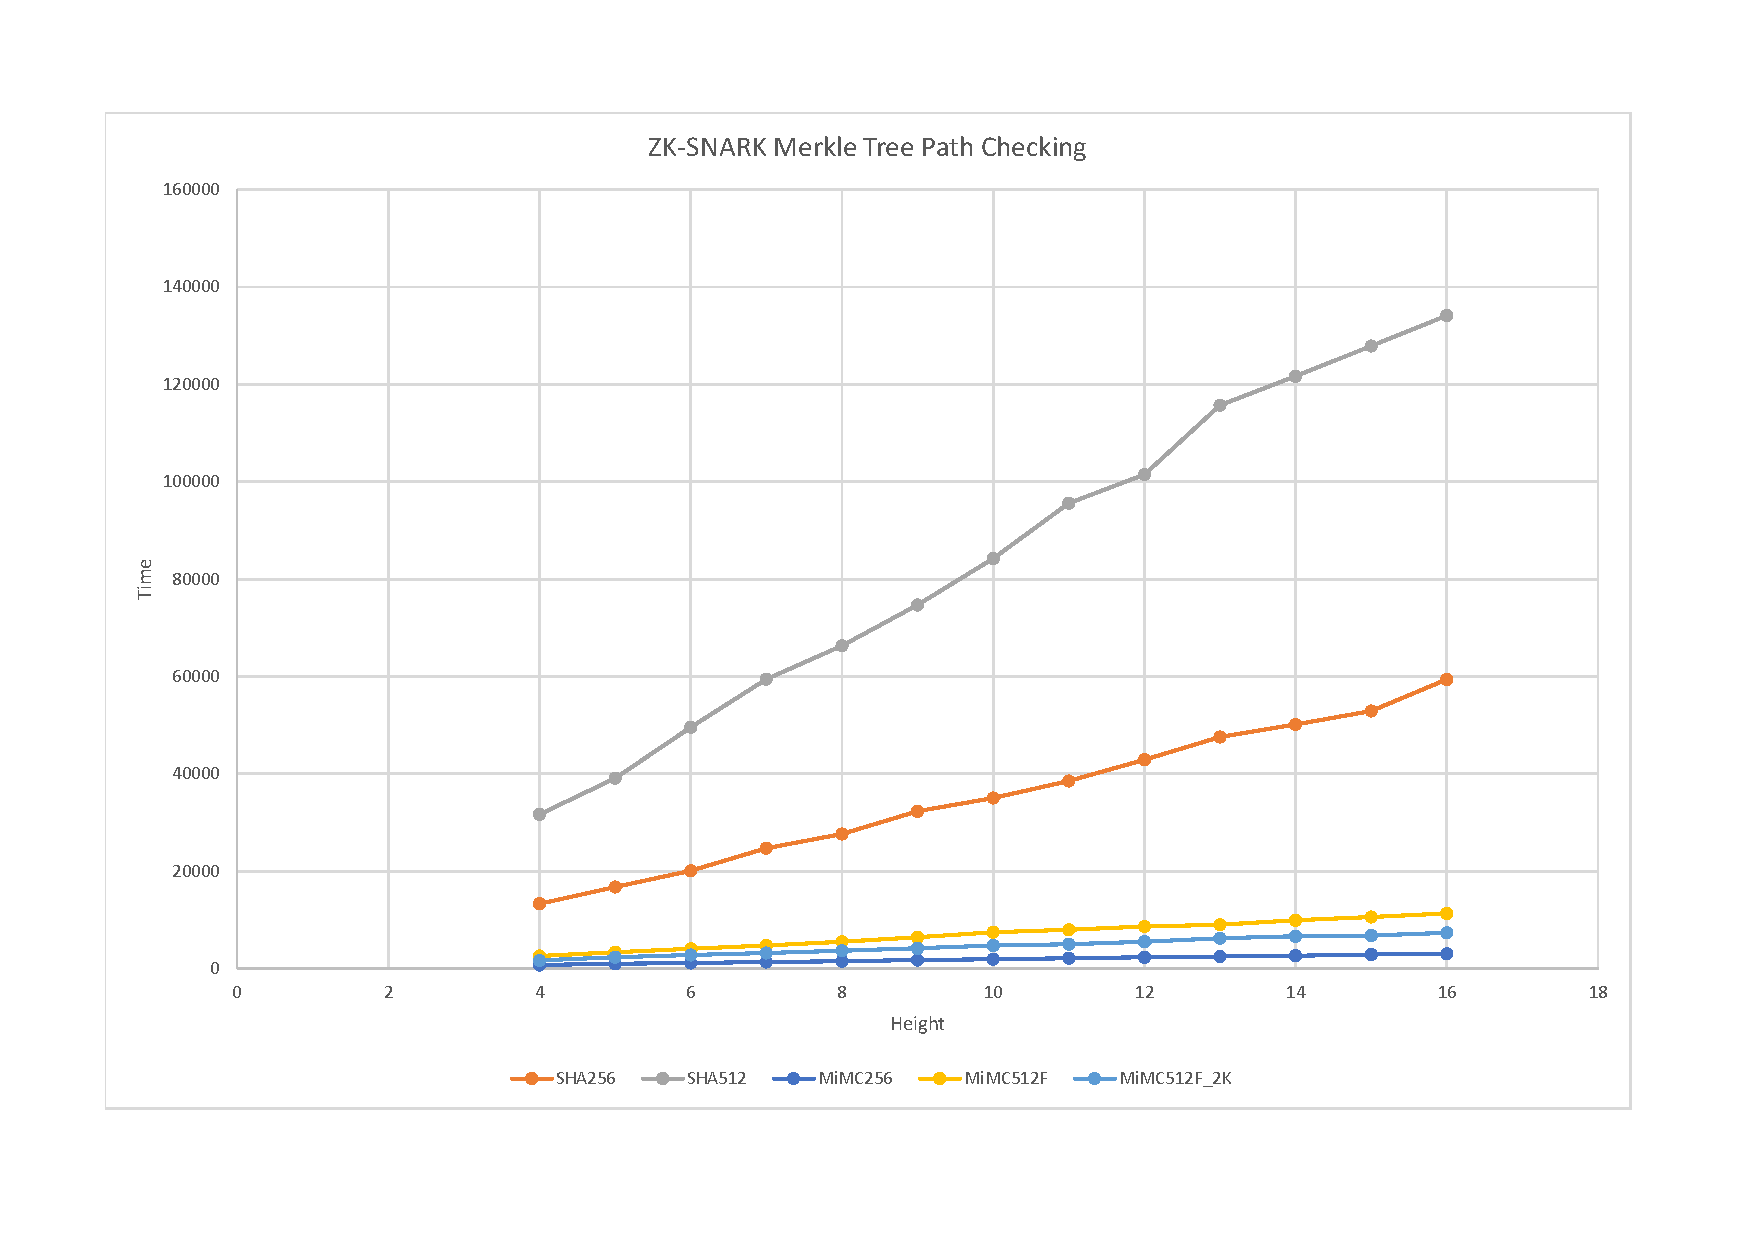
\includegraphics[scale=0.33]{res/mtree_total.pdf}
	\caption{Total time (in ms) required for synthesizing and solving a ZK-SNARK Merkle Tree path
		veritication circuit at varying heights.}\label{fig:mtree_total}
\end{figure}

Figure~\ref{fig:mtree_total} shows the total time, in milliseconds, required to create an
arithmetic circuit for Merkle tree path verification, convert it to R1CS, build the QAP and the
proof, and verify the proof, using different underlying hash functions.
As expected, MiMC-256 is the fastest one, followed by double-key MiMC-512F and single-key MiMC-512F
in the respective order, with SHA-256 and SHA-512 being extremely slower.
\begin{figure}
	\centering
	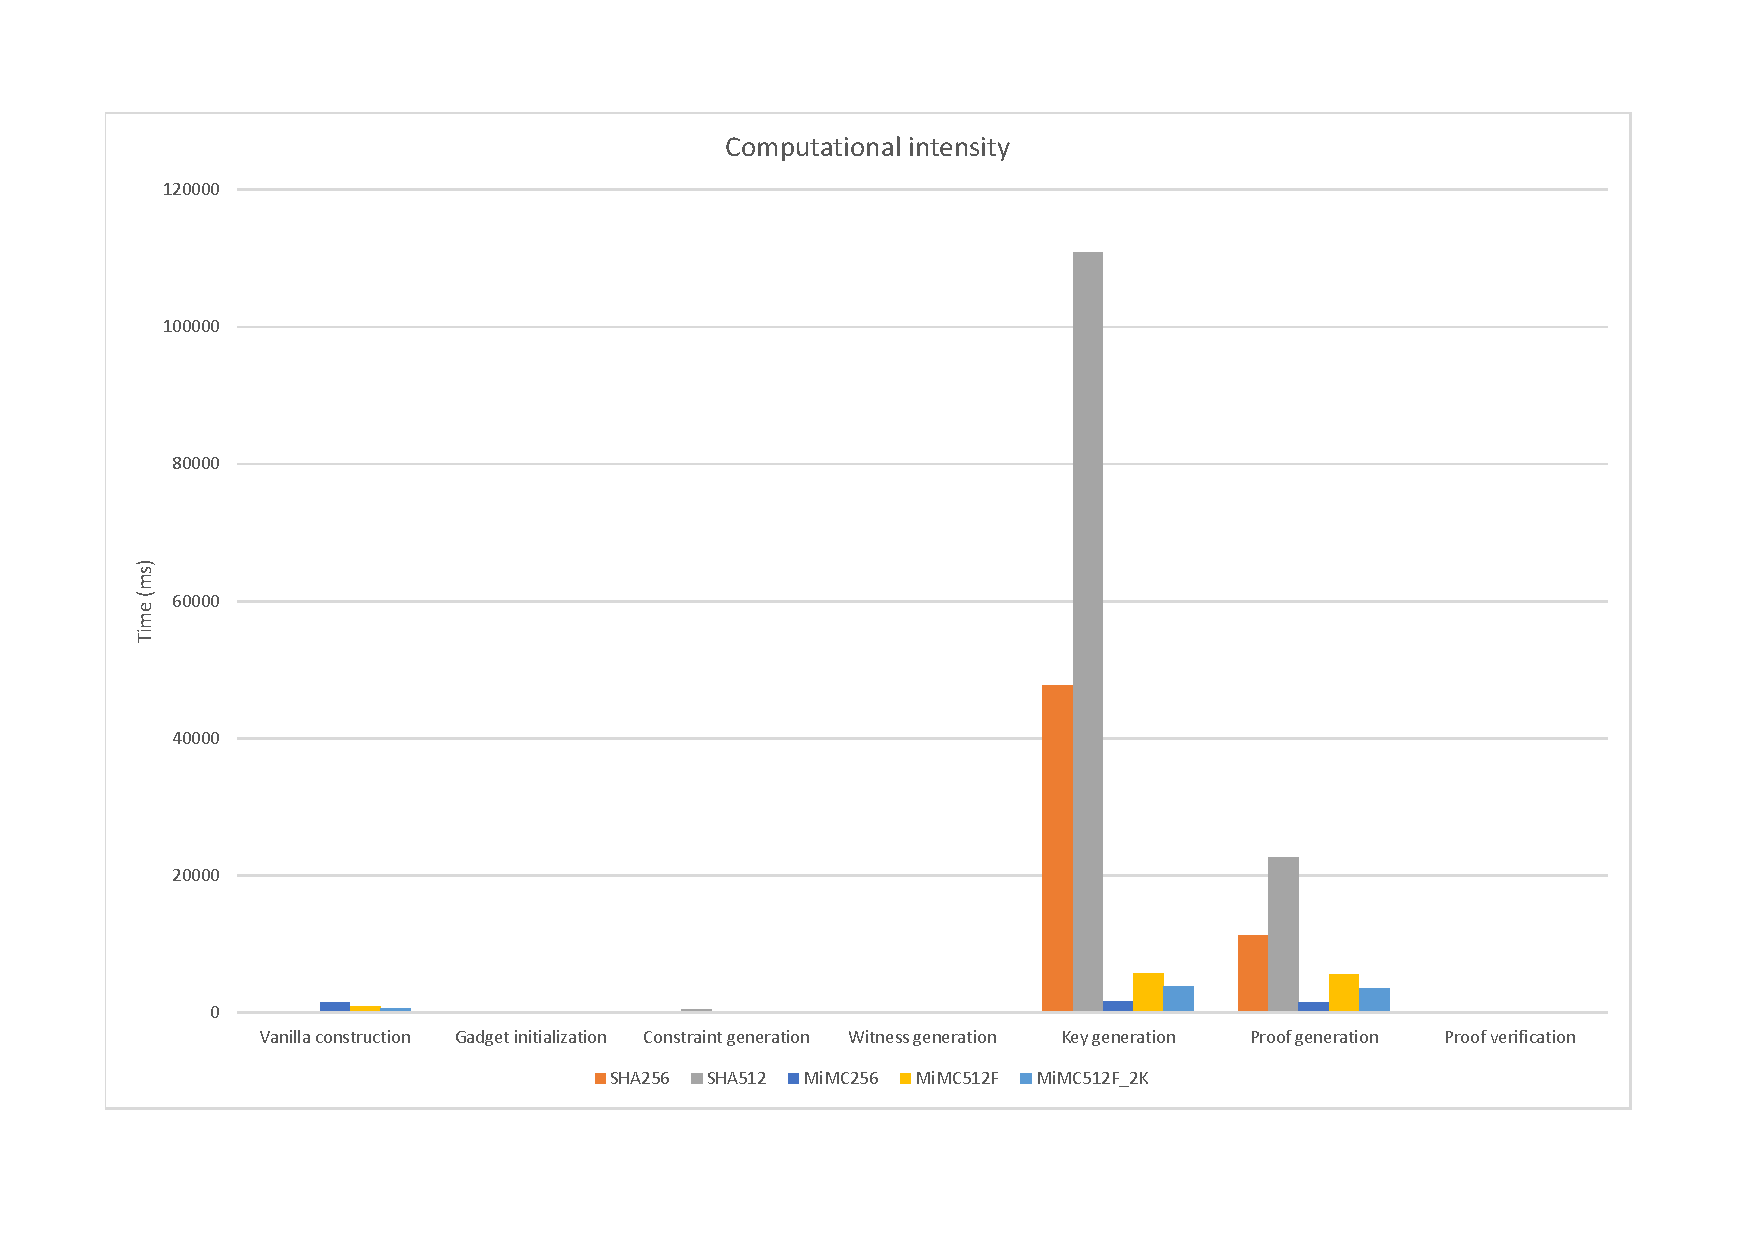
\includegraphics[scale=0.33]{res/mtree_intensity.pdf}
	\caption{Computational intensity of the various phases of the ZK-SNARK protocol: key and proof
		generation dominate the cost.}\label{fig:mtree_intensity}
\end{figure}

Figure~\ref{fig:mtree_intensity} shows the computational intensity of the different parts of the
Pinocchio protocol: since key and proof generation times completely dominate the cost, and these
are transparent to the library user, it is extremely important to optimize the arithmetic circuit
layout, even if it makes the synthesizing code more complex.
\begin{figure}
	\centering
	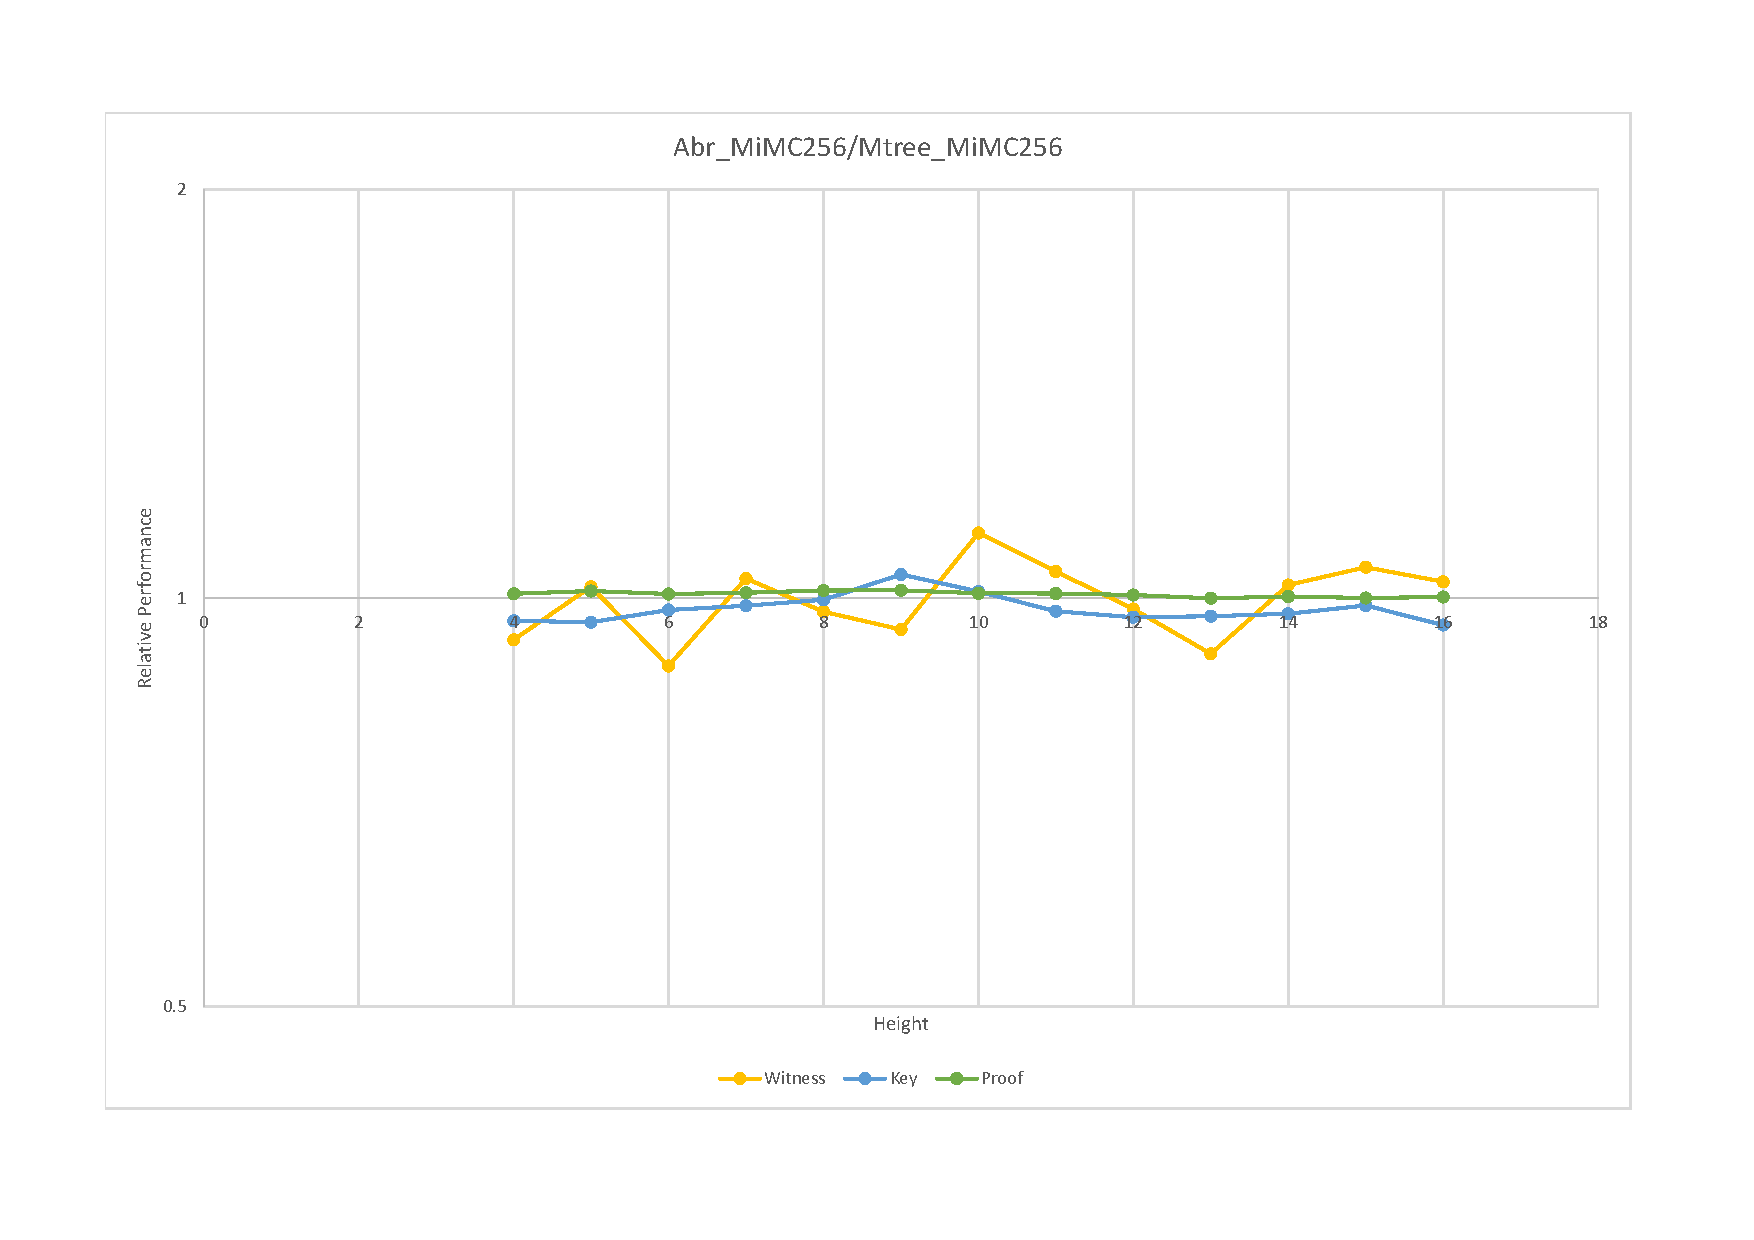
\includegraphics[scale=0.33]{res/mtree_vs_abr.pdf}
	\caption{Relative performance of path verification over ABRs compared to Merkle Trees using
		MiMC-256; we can see that the difference is negligible.}\label{fig:mtree_vs_abr}
\end{figure}

Finally, in Figure~\ref{fig:mtree_vs_abr} we compared the performance of path verification over
ABRs compared to Merkle Trees when using a field-native CHF like MiMC-256.
The difference, as expected, is negligible, and even for non-native functions like SHA-256, the
Merkle Tree is about 10--20\% faster than the ABR\@.


\section{Conclusions and future directions}\label{sec:conclusions}
\end{document}
